\documentclass[10pt]{article}
\usepackage{xstring}
\usepackage{tikz}
\usetikzlibrary{calc}
\newcommand{\Size}{3.25cm}
\tikzset{Square/.style={
inner sep=0pt,
text width=\Size, 
minimum size=\Size,
draw=black,
align=center,
}
}
\begin{document}
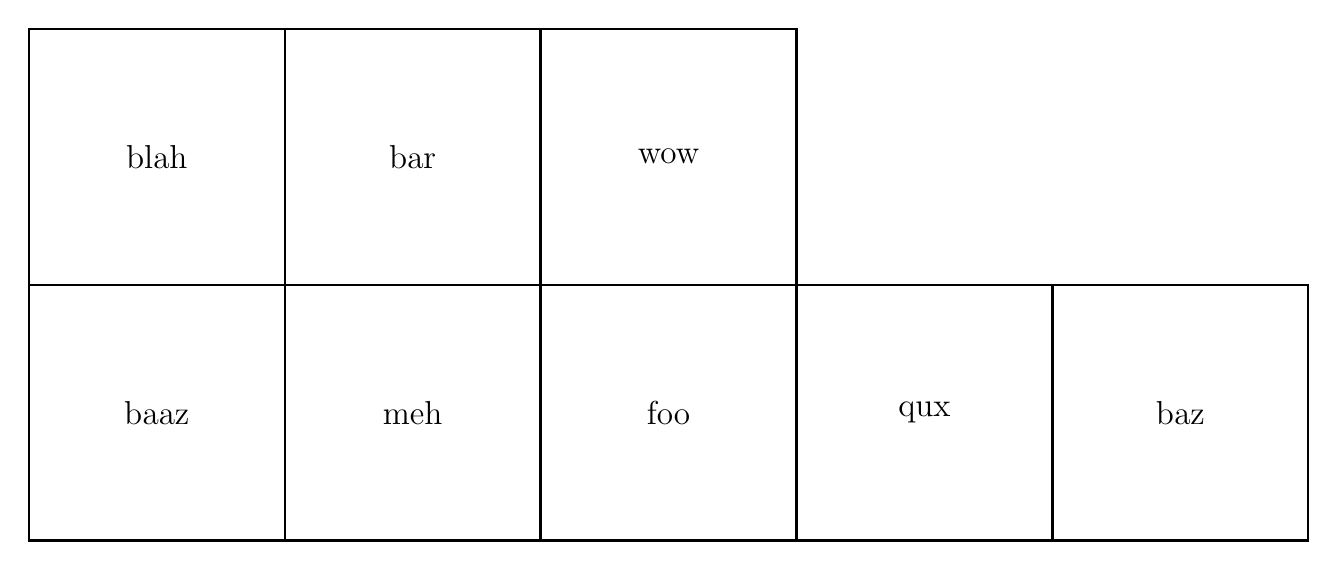
\begin{tikzpicture}[draw=black, thick, x=\Size,y=\Size]
\node [Square] at ($(0, 0)-(0.5,0.5)$) {\large baaz};\node [Square] at ($(1, 0)-(0.5,0.5)$) {\large meh};\node [Square] at ($(2, 0)-(0.5,0.5)$) {\large foo};\node [Square] at ($(3, 0)-(0.5,0.5)$) {\large qux};\node [Square] at ($(4, 0)-(0.5,0.5)$) {\large baz};\node [Square] at ($(0, 1)-(0.5,0.5)$) {\large blah};\node [Square] at ($(1, 1)-(0.5,0.5)$) {\large bar};\node [Square] at ($(2, 1)-(0.5,0.5)$) {\large wow};\end{tikzpicture}
\end{document}
